%% bare_conf.tex
%% V1.4b
%% 2015/08/26
%% by Michael Shell
%% See:
%% http://www.michaelshell.org/
%% for current contact information.
%%
%% This is a skeleton file demonstrating the use of IEEEtran.cls
%% (requires IEEEtran.cls version 1.8b or later) with an IEEE
%% conference paper.
%%
%% Support sites:
%% http://www.michaelshell.org/tex/ieeetran/
%% http://www.ctan.org/pkg/ieeetran
%% and
%% http://www.ieee.org/
%%*************************************************************************
%% Legal Notice:
%% This code is offered as-is without any warranty either expressed or
%% implied; without even the implied warranty of MERCHANTABILITY or
%% FITNESS FOR A PARTICULAR PURPOSE! 
%% User assumes all risk.
%% In no event shall the IEEE or any contributor to this code be liable for
%% any damages or losses, including, but not limited to, incidental,
%% consequential, or any other damages, resulting from the use or misuse
%% of any information contained here.
%%
%% All comments are the opinions of their respective authors and are not
%% necessarily endorsed by the IEEE.
%%
%% This work is distributed under the LaTeX Project Public License (LPPL)
%% ( http://www.latex-project.org/ ) version 1.3, and may be freely used,
%% distributed and modified. A copy of the LPPL, version 1.3, is included
%% in the base LaTeX documentation of all distributions of LaTeX released
%% 2003/12/01 or later.
%% Retain all contribution notices and credits.
%% ** Modified files should be clearly indicated as such, including  **
%% ** renaming them and changing author support contact information. **
%%*************************************************************************


% *** Authors should verify (and, if needed, correct) their LaTeX system  ***
% *** with the testflow diagnostic prior to trusting their LaTeX platform ***
% *** with production work. The IEEE's font choices and paper sizes can   ***
% *** trigger bugs that do not appear when using other class files.       ***                          
% The testflow support page is at:
% http://www.michaelshell.org/tex/testflow/

\documentclass[conference]{IEEEtran}
% Some Computer Society conferences also require the compsoc mode option,
% but others use the standard conference format.
%
% If IEEEtran.cls has not been installed into the LaTeX system files,
% manually specify the path to it like:
% \documentclass[conference]{../sty/IEEEtran}

\usepackage{booktabs}
\newcommand{\ra}[1]{\renewcommand{\arraystretch}{#1}}

\usepackage[usenames,dvipsnames]{color}
\newcommand{\todo}[1]
  {{\scriptsize \textbf{\color{red} {#1}}}}



% Some very useful LaTeX packages include:
% (uncomment the ones you want to load)


% *** MISC UTILITY PACKAGES ***
%
%\usepackage{ifpdf}
% Heiko Oberdiek's ifpdf.sty is very useful if you need conditional
% compilation based on whether the output is pdf or dvi.
% usage:
% \ifpdf
%   % pdf code
% \else
%   % dvi code
% \fi
% The latest version of ifpdf.sty can be obtained from:
% http://www.ctan.org/pkg/ifpdf
% Also, note that IEEEtran.cls V1.7 and later provides a builtin
% \ifCLASSINFOpdf conditional that works the same way.
% When switching from latex to pdflatex and vice-versa, the compiler may
% have to be run twice to clear warning/error messages.


\usepackage{listings}



% *** CITATION PACKAGES ***
%
\usepackage{cite}
% cite.sty was written by Donald Arseneau
% V1.6 and later of IEEEtran pre-defines the format of the cite.sty package
% \cite{} output to follow that of the IEEE. Loading the cite package will
% result in citation numbers being automatically sorted and properly
% "compressed/ranged". e.g., [1], [9], [2], [7], [5], [6] without using
% cite.sty will become [1], [2], [5]--[7], [9] using cite.sty. cite.sty's
% \cite will automatically add leading space, if needed. Use cite.sty's
% noadjust option (cite.sty V3.8 and later) if you want to turn this off
% such as if a citation ever needs to be enclosed in parenthesis.
% cite.sty is already installed on most LaTeX systems. Be sure and use
% version 5.0 (2009-03-20) and later if using hyperref.sty.
% The latest version can be obtained at:
% http://www.ctan.org/pkg/cite
% The documentation is contained in the cite.sty file itself.
\lstset{language=Java}
\definecolor{dkgreen}{rgb}{0,0.5,0}
\definecolor{dkred}{rgb}{0.5,0,0}
\definecolor{gray}{rgb}{0.5,0.5,0.5}
\lstset{
basicstyle=\ttfamily\bfseries\scriptsize,
  morekeywords={virtualinvoke}, 
  keywordstyle=\color{blue},
  ndkeywordstyle=\color{red},
  commentstyle=\color{dkred},
  stringstyle=\color{dkgreen},
  numbers=left,
  breaklines=true,
  numberstyle=\ttfamily\footnotesize\color{gray},
  stepnumber=1,
  numbersep=10pt,
  backgroundcolor=\color{white},
  tabsize=4,
  showspaces=false,
  frame=bt,
  showstringspaces=false,
  xleftmargin=.23in,
  moredelim=[is][\color{red}]{@}{@}, deletekeywords={}, captionpos=b, belowskip=1pt
}






% *** GRAPHICS RELATED PACKAGES ***
%
\ifCLASSINFOpdf
   \usepackage[pdftex]{graphicx}
  % declare the path(s) where your graphic files are
   \graphicspath{{images/}}
  % and their extensions so you won't have to specify these with
  % every instance of \includegraphics
   \DeclareGraphicsExtensions{.pdf,.jpeg,.png, .jpg}
\else
  % or other class option (dvipsone, dvipdf, if not using dvips). graphicx
  % will default to the driver specified in the system graphics.cfg if no
  % driver is specified.
  % \usepackage[dvips]{graphicx}
  % declare the path(s) where your graphic files are
  % \graphicspath{{../eps/}}
  % and their extensions so you won't have to specify these with
  % every instance of \includegraphics
  % \DeclareGraphicsExtensions{.eps}
\fi
% graphicx was written by David Carlisle and Sebastian Rahtz. It is
% required if you want graphics, photos, etc. graphicx.sty is already
% installed on most LaTeX systems. The latest version and documentation
% can be obtained at: 
% http://www.ctan.org/pkg/graphicx
% Another good source of documentation is "Using Imported Graphics in
% LaTeX2e" by Keith Reckdahl which can be found at:
% http://www.ctan.org/pkg/epslatex
%
% latex, and pdflatex in dvi mode, support graphics in encapsulated
% postscript (.eps) format. pdflatex in pdf mode supports graphics
% in .pdf, .jpeg, .png and .mps (metapost) formats. Users should ensure
% that all non-photo figures use a vector format (.eps, .pdf, .mps) and
% not a bitmapped formats (.jpeg, .png). The IEEE frowns on bitmapped formats
% which can result in "jaggedy"/blurry rendering of lines and letters as
% well as large increases in file sizes.
%
% You can find documentation about the pdfTeX application at:
% http://www.tug.org/applications/pdftex





% *** MATH PACKAGES ***
%
\usepackage{amsmath}
% A popular package from the American Mathematical Society that provides
% many useful and powerful commands for dealing with mathematics.
%
% Note that the amsmath package sets \interdisplaylinepenalty to 10000
% thus preventing page breaks from occurring within multiline equations. Use:
%\interdisplaylinepenalty=2500
% after loading amsmath to restore such page breaks as IEEEtran.cls normally
% does. amsmath.sty is already installed on most LaTeX systems. The latest
% version and documentation can be obtained at:
% http://www.ctan.org/pkg/amsmath





% *** SPECIALIZED LIST PACKAGES ***
%
%\usepackage{algorithmic}
% algorithmic.sty was written by Peter Williams and Rogerio Brito.
% This package provides an algorithmic environment fo describing algorithms.
% You can use the algorithmic environment in-text or within a figure
% environment to provide for a floating algorithm. Do NOT use the algorithm
% floating environment provided by algorithm.sty (by the same authors) or
% algorithm2e.sty (by Christophe Fiorio) as the IEEE does not use dedicated
% algorithm float types and packages that provide these will not provide
% correct IEEE style captions. The latest version and documentation of
% algorithmic.sty can be obtained at:
% http://www.ctan.org/pkg/algorithms
% Also of interest may be the (relatively newer and more customizable)
% algorithmicx.sty package by Szasz Janos:
% http://www.ctan.org/pkg/algorithmicx




% *** ALIGNMENT PACKAGES ***
%
%\usepackage{array}
% Frank Mittelbach's and David Carlisle's array.sty patches and improves
% the standard LaTeX2e array and tabular environments to provide better
% appearance and additional user controls. As the default LaTeX2e table
% generation code is lacking to the point of almost being broken with
% respect to the quality of the end results, all users are strongly
% advised to use an enhanced (at the very least that provided by array.sty)
% set of table tools. array.sty is already installed on most systems. The
% latest version and documentation can be obtained at:
% http://www.ctan.org/pkg/array


% IEEEtran contains the IEEEeqnarray family of commands that can be used to
% generate multiline equations as well as matrices, tables, etc., of high
% quality.




% *** SUBFIGURE PACKAGES ***
%\ifCLASSOPTIONcompsoc
%  \usepackage[caption=false,font=normalsize,labelfont=sf,textfont=sf]{subfig}
%\else
%  \usepackage[caption=false,font=footnotesize]{subfig}
%\fi
% subfig.sty, written by Steven Douglas Cochran, is the modern replacement
% for subfigure.sty, the latter of which is no longer maintained and is
% incompatible with some LaTeX packages including fixltx2e. However,
% subfig.sty requires and automatically loads Axel Sommerfeldt's caption.sty
% which will override IEEEtran.cls' handling of captions and this will result
% in non-IEEE style figure/table captions. To prevent this problem, be sure
% and invoke subfig.sty's "caption=false" package option (available since
% subfig.sty version 1.3, 2005/06/28) as this is will preserve IEEEtran.cls
% handling of captions.
% Note that the Computer Society format requires a larger sans serif font
% than the serif footnote size font used in traditional IEEE formatting
% and thus the need to invoke different subfig.sty package options depending
% on whether compsoc mode has been enabled.
%
% The latest version and documentation of subfig.sty can be obtained at:
% http://www.ctan.org/pkg/subfig




% *** FLOAT PACKAGES ***
%
%\usepackage{fixltx2e}
% fixltx2e, the successor to the earlier fix2col.sty, was written by
% Frank Mittelbach and David Carlisle. This package corrects a few problems
% in the LaTeX2e kernel, the most notable of which is that in current
% LaTeX2e releases, the ordering of single and double column floats is not
% guaranteed to be preserved. Thus, an unpatched LaTeX2e can allow a
% single column figure to be placed prior to an earlier double column
% figure.
% Be aware that LaTeX2e kernels dated 2015 and later have fixltx2e.sty's
% corrections already built into the system in which case a warning will
% be issued if an attempt is made to load fixltx2e.sty as it is no longer
% needed.
% The latest version and documentation can be found at:
% http://www.ctan.org/pkg/fixltx2e


%\usepackage{stfloats}
% stfloats.sty was written by Sigitas Tolusis. This package gives LaTeX2e
% the ability to do double column floats at the bottom of the page as well
% as the top. (e.g., "\begin{figure*}[!b]" is not normally possible in
% LaTeX2e). It also provides a command:
%\fnbelowfloat
% to enable the placement of footnotes below bottom floats (the standard
% LaTeX2e kernel puts them above bottom floats). This is an invasive package
% which rewrites many portions of the LaTeX2e float routines. It may not work
% with other packages that modify the LaTeX2e float routines. The latest
% version and documentation can be obtained at:
% http://www.ctan.org/pkg/stfloats
% Do not use the stfloats baselinefloat ability as the IEEE does not allow
% \baselineskip to stretch. Authors submitting work to the IEEE should note
% that the IEEE rarely uses double column equations and that authors should try
% to avoid such use. Do not be tempted to use the cuted.sty or midfloat.sty
% packages (also by Sigitas Tolusis) as the IEEE does not format its papers in
% such ways.
% Do not attempt to use stfloats with fixltx2e as they are incompatible.
% Instead, use Morten Hogholm'a dblfloatfix which combines the features
% of both fixltx2e and stfloats:
%
% \usepackage{dblfloatfix}
% The latest version can be found at:
% http://www.ctan.org/pkg/dblfloatfix


\usepackage{verbatim}
\usepackage{amsmath}
\usepackage{amsfonts}
\usepackage{amssymb}
\usepackage{graphicx}

% INCLUDE THIS
\usepackage{listings, lstautogobble}

% *** PDF, URL AND HYPERLINK PACKAGES ***
%
\usepackage{url}
% url.sty was written by Donald Arseneau. It provides better support for
% handling and breaking URLs. url.sty is already installed on most LaTeX
% systems. The latest version and documentation can be obtained at:
% http://www.ctan.org/pkg/url
% Basically, \url{my_url_here}.




% *** Do not adjust lengths that control margins, column widths, etc. ***
% *** Do not use packages that alter fonts (such as pslatex).         ***
% There should be no need to do such things with IEEEtran.cls V1.6 and later.
% (Unless specifically asked to do so by the journal or conference you plan
% to submit to, of course. )


% correct bad hyphenation here
\hyphenation{op-tical net-works semi-conduc-tor}

\usepackage{microtype}
\usepackage{lipsum}
\usepackage{multicol}

\usepackage{array}
\usepackage{tabulary}
\newcolumntype{K}[1]{>{\arraybackslash}p{#1}}

\usepackage{array}
\newcolumntype{C}[1]{>{\centering\arraybackslash}m{#1}}
\newcolumntype{R}[1]{>{\raggedleft\arraybackslash}m{#1}}

\usepackage{adjustbox}

 
\pagenumbering{arabic}
\begin{document}
%
% paper title
% Titles are generally capitalized except for words such as a, an, and, as,
% at, but, by, for, in, nor, of, on, or, the, to and up, which are usually
% not capitalized unless they are the first or last word of the title.
% Linebreaks  can be used within to get better formatting as desired.
% Do not put math or special symbols in the title.
\title{Using a probabilistic model to predict bug fixes}


% author names and affiliations
% use a multiple column layout for up to three different
% affiliations

\author{\IEEEauthorblockN{Authors hidden for the purposes of double blind review}
%\IEEEauthorblockA{\\
%\\
%\\}

%REPLACE FOR CAMERA READY:
%\author{\IEEEauthorblockN{Mauricio Soto}
%\IEEEauthorblockA{Carnegie Mellon University\\
%Pittsburgh PA\\
%mauriciosoto@cmu.edu}
%\and
%\IEEEauthorblockN{Claire Le Goues}
%\IEEEauthorblockA{Carnegie Mellon University\\
%Pittsburgh PA\\
%clegoues@cs.cmu.edu}




%\and
%\IEEEauthorblockN{James Kirk\\ and Montgomery Scott}
%\IEEEauthorblockA{Starfleet Academy\\
%San Francisco, California 96678--2391\\
%Telephone: (800) 555--1212\\
%Fax: (888) 555--1212}

}

% conference papers do not typically use \thanks and this command
% is locked out in conference mode. If really needed, such as for
% the acknowledgment of grants, issue a \IEEEoverridecommandlockouts
% after \documentclass

% for over three affiliations, or if they all won't fit within the width
% of the page, use this alternative format:
% 
%\author{\IEEEauthorblockN{Michael Shell\IEEEauthorrefmark{1},
%Homer Simpson\IEEEauthorrefmark{2},
%James Kirk\IEEEauthorrefmark{3}, 
%Montgomery Scott\IEEEauthorrefmark{3} and
%Eldon Tyrell\IEEEauthorrefmark{4}}
%\IEEEauthorblockA{\IEEEauthorrefmark{1}School of Electrical and Computer Engineering\\
%Georgia Institute of Technology,
%Atlanta, Georgia 30332--0250\\ Email: see http://www.michaelshell.org/contact.html}
%\IEEEauthorblockA{\IEEEauthorrefmark{2}Twentieth Century Fox, Springfield, USA\\
%Email: homer@thesimpsons.com}
%\IEEEauthorblockA{\IEEEauthorrefmark{3}Starfleet Academy, San Francisco, California 96678-2391\\
%Telephone: (800) 555--1212, Fax: (888) 555--1212}
%\IEEEauthorblockA{\IEEEauthorrefmark{4}Tyrell Inc., 123 Replicant Street, Los Angeles, California 90210--4321}}




% use for special paper notices
%\IEEEspecialpapernotice{(Invited Paper)}




% make the title area
\maketitle

% As a general rule, do not put math, special symbols or citations
% in the abstract
\begin{abstract}
Automatic Software Repair (APR) has significant potential to reduce software
maintenance costs by reducing the human effort required to localize and fix
bugs. Well-known state-of-the-art generate-and-validate 
APR approaches select between and instantiate various mutation operators
to construct candidate patches, informed by largely heuristic probability
distributions.  This may reduce effectiveness in terms of both efficiency and
output quality: patches informed by the ways humans fix bugs may be considered
more acceptable.  In practice, human developers
have many options in terms of how to edit code to fix bugs, some of which 
are far more common than others (e.g., deleting a line of code is more common
than adding a new class).
Treating such edits as 
APR mutation operators, we  
mined the most recent 100 bug-fixing commits from each of the 500 most popular Java projects in Github (largest 
dataset to date) to
create a probabilistic model describing edit distributions.
We categorize, compare and evaluate the different mutation operators used in 
the state of the art approaches. Finally, we mine association rules to analyze context surrounding
multi-edit source code changes, an understudied problem 
that covers the majority of real source code changes. Our evaluation
indicates that by applying the probabilistic model we are able to find
the correct mutation operator to patch bugs faster in the majority of bugs
studied, and that using the superset of all mutation operators performs better than restricting the mutation operator pool to just one category.  
\end{abstract}


% no keywords




% For peer review papers, you can put extra information on the cover
% page as needed:
% \ifCLASSOPTIONpeerreview
% \begin{center} \bfseries EDICS Category: 3-BBND \end{center}
% \fi
%
% For peerreview papers, this IEEEtran command inserts a page break and
% creates the second title. It will be ignored for other modes.
\IEEEpeerreviewmaketitle



\section{Introduction} \label{introduction}
% no \IEEEPARstart
Repairing errors is one of the most 
resource intensive tasks in 
the software development process~\cite{Weiss07,Tassey02,Britton13}, especially for large, real-world systems~\cite{Liblit03,Anvik05}.
%
Significant recent research effort has been dedicated to
building automatic program repair (APR) tools that are able to address
bugs in 
programs (e.g.~\cite{legoues12,kim2013,Weimer13,long15SPR,long16proph,debroy10,perkins09,wei10}).

One well-known class of repair techniques follows a 
\emph{generate-and-validate} approach  (e.g., GenProg~\cite{legoues12}, 
Par~\cite{kim2013}, TrpAutoRepair~\cite{Qi13TrpAutoR}
Prophet~\cite{long16proph}, HDRepair~\cite{xuan16}), which takes as input a test suite, 
including at
least one failing test case exposing
a defect, and source code to be 
modified.  These approaches then \emph{generate} a large patch candidate space 
by applying 
mutation operators to the original source code and \emph{validate} each by
running the potentially patched program against the test suite, seeking a candidate that
leads the program to pass all input test cases. 

The search space of possible patches that can repair any bug is trivially
infinite.  The nature of this search space introduces key tensions in APR
technique design.  First, 
techniques must manage the space carefully so as to traverse it in a scalable and
effective manner.  One way that current techniques manage this problem is to
only consider a limited set of of possible changes, or \emph{mutation operators}, 
to apply to the code.
There is a broad diversity of such operators used in automatic program repair, such as deleting or inserting 
statements~\cite{legoues12}, applying templates~\cite{kim2013}, transformation 
schemas~\cite{long16proph,long15SPR}, etc.\footnote{In this study, we exclude 
from consideration semantic approaches, as we focus on
candidate patches creation in the heuristic or syntactic context.} 
Given a potentially-faulty location (typically identified using off-the-shelf fault
localization, e.g. Tarantula~\cite{Jones02}), these APR  approaches further use heuristics or
heuristically-informed probability distributions to select between
mutation operators when constructing candidate patches.

However, even with these heuristics and design choices, the search space of candidate
repairs for many bugs remains intractably large.  Most techniques are thus
limited by design to producing single-edit patches (e.g., TrpAutoRepair~\cite{Qi13TrpAutoR}). 
Those few that can theoretically produce multi-edit patches
(e.g., GenProg~\cite{legoues12}) typically still only produce small changes in
practice~\cite{Qi15,arcuri11}. 
Indeed, patches
consisting of several mutations are undertreated in the APR context, even though the vast majority
of patches in existence are comprised of multiple edits~\cite{Soto16,zhong15}.

These attempts to tackle scalability are in tension with a second major concern
in APR research: the quality of the generated patches~\cite{Qi15}.  One way to
improve output quality is to use more expressive mutation operators to produce a
richer search space~\cite{long16}.  However, more and more expressive mutation
operators increase the size of the 
space, and not always in a way that supports the construction of more correct
patches.  Thus, although APR techniques would benefit from more expressive
operators, they cannot do so without a way to choose between them that manages
the search space explosion problem, ideally all while increasing the probability
of finding correct patches.

Fundamentally, in bug-fixing reality, human developers use
certain mutation operators much more often than others (e.g., adding an \emph{IfStatement} is more common than adding a \emph{TypeDeclarationStatement})~\cite{Soto16}. In this
work, we propose to study
and then systematically simulate the behavior of human developers to create
patches. This idea has been leveraged manually in the past to create
mutation operators that produce more human-acceptable patches~\cite{kim2013} and
to inform patch \emph{ranking} (rather than
construction) when traversing the search space~\cite{xuan16,long16proph}. 
Our primary supposition is that our approach can scalably support a richer
search space constructed via more expressive mutation operators that are more
likely to produce high-quality patches.  

To this end, we mine bug fixing commits from 
the 500 most popular Github Java projects to model the selection probability of
the possible mutation operators based on 
empirical data that describes how human programmers fix their code.  
The APR search space, including the various mutation
operators used by different techniques, has been growing in a relatively ad hoc 
manner.  We mitigate this effect by categorizing and comparing a superset of
mutation operators in use in a number of 
state-of-the-art approaches.
We use the constructed model to inform a repair approach that chooses from the set of possible
operators based on these real-world incidences.
As a result, we go beyond prior work  by generalizing
to a broader and more expressive set of
mutation operators, and using a fully-automatically-mined probability model much 
earlier in the APR process, when patch candidates are actually \emph{created.}
Furthermore, we propose and initially validate a new approach for modeling
multi-edit repairs based on mining previous rules from historical edit data, 
predicting from a given 
single-edit mutation which operation should be applied
next.  This serves  as a first step towards
scalable traversal of the multi-edit patch space. 

We evaluate the predictive power of our mined models on their own, in terms of their
accuracy in predicting the operators used in real-world bug fixes.  We also
integrate the single-edit model into a new repair algorithm that we demonstrate
in comparison to several previous techniques on a subset of real-world defects from Defects4j~\cite{just14}. 
%
The primary contributions of this paper thus are:
\begin{itemize}
\item \textbf{Empirical model of single-edit repairs to Java code} mined
      from the 100 most recent bug fixes from the 500 most popular Java projects on
    Github. This study also provides a deeper
    understanding of which mutation operators are used by programmers to fix
    errors in source code.
	\item \textbf{New Repair Approach}, which uses mutation operators
    from multiple state-of-the-art approaches and
    the above-mentioned models to choose between them, favoring those more commonly
    used by human developers.
    \item \textbf{Development and integration} of this approach for the Java programming language in a tool, available online, which can apply the several different mutation operators, and the probabilistic model discussed in this study.\footnote{We will release all artifacts, code, and data associated with this publication post blind-review.} %\footnote{https://bitbucket.org/clegoues/genprog4java}
  \item \textbf{Evaluation} of the probabilistic model in several
    contexts, including as part of a new APR approach used to repair real world bugs from well
    known open source projects (independent of those used to inform model
    construction). We independently evaluate generate patch quality using a held-out test
    suite. We conclude that by creating candidate patches using human behavior
    we are able to find patches faster than a technique that does not use such
    mined probabilities, and that the patch creation
    process benefits from combining mutation operator categories.  We compare
    our approach to several state-of-the-art approaches in terms of patch
    success and quality. 
  \item \textbf{Multi-edit repair approach} A proposed technique, and an initial
    validation thereof, to construct 
    bug-fixing patches requiring several mutations by mining and then applying association
    rules from a large set of historical bug fixes. 
\end{itemize}

The rest of this paper proceeds as follows: We first outline
generate-and-validate repair and, in particular, 
categorize and generalize the mutation operators used in state of the art
approaches (Section~\ref{background}). Section~\ref{buildingTheModel}
describes our approach to building probabilistic models of human 
edits for both single- and multi-edit bug fixes. Section~\ref{evaluation}
describes our evaluation. Section~\ref{relatedWork} describes
related work; Section~\ref{conclusion} concludes. 

\section{Generate-and-validate repair and operators} 
\label{background}

In this section, we outline generate and validate repair at a high level
(Section~\ref{sec-paradigm}), to provide the necessary background to understand our
work, and then detail and categorize the mutation operators used in the
state-of-the-art and that we model, mine, and leverage in our approach
(Section~\ref{categorization}).  
 
 
\subsection{Paradigm}
\label{sec-paradigm}


Figure~\ref{fig:generateandvalidate} outlines the general paradigm for generate-and-validate repair. This approach starts with source code with one or more bugs and a test suite. The test suite contains passing
test cases to witness the correct program behavior, and failing test 
cases exposing the behavior to be repaired.

\begin{figure}[!h]
  \centering
    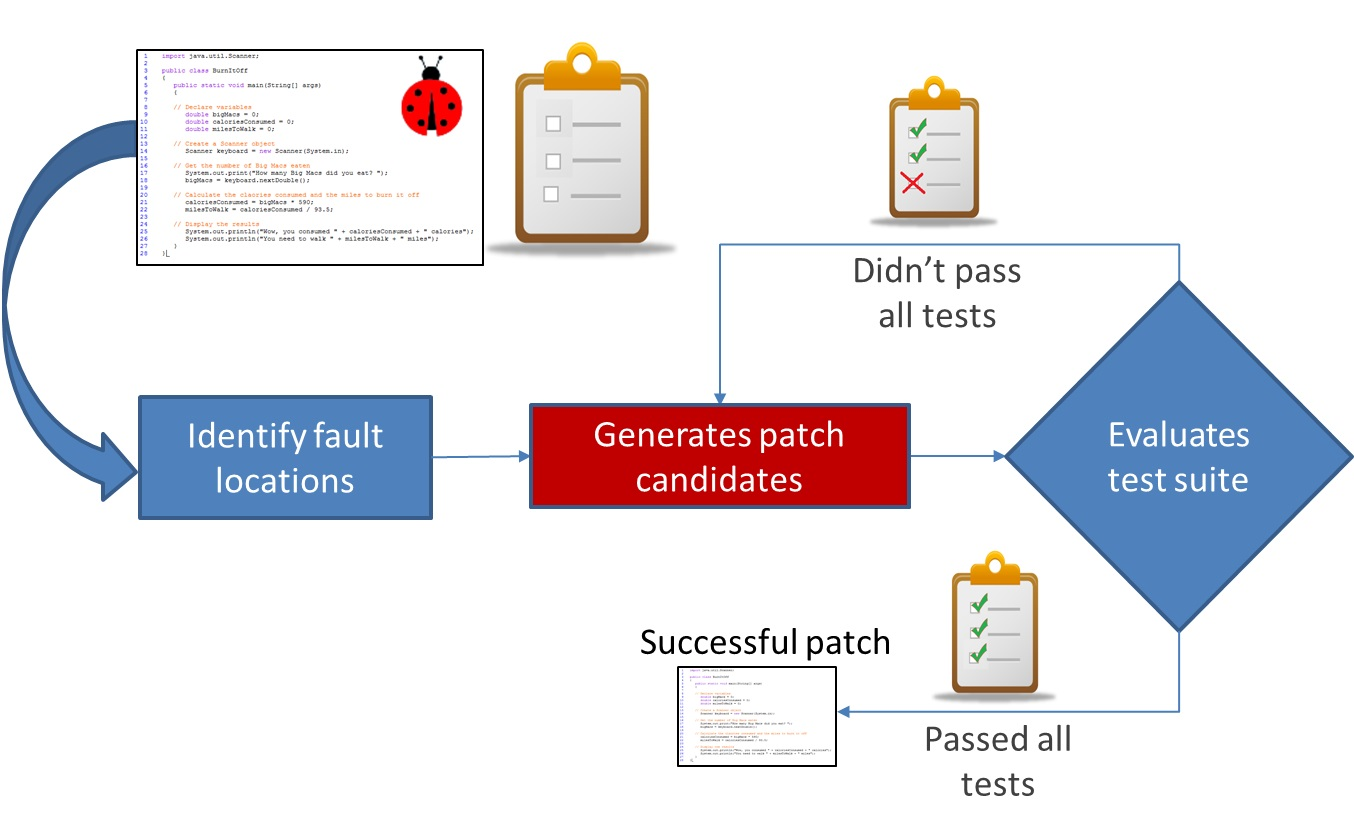
\includegraphics[scale=0.25]{Picture1}
  \caption{Generate and validate approach}
  \label{fig:generateandvalidate}
\end{figure}

Given the inputs, a generic generate-and-validate APR approach
localizes the error to a smaller set of
candidate program statements (typically using an off-the-shelf approach, e.g. Tarantula~\cite{Jones02}). 
Candidate patches are produced by modifying the program at identified faulty 
statements. To 
create such a candidate patch, these techniques typically identify a subset of
a given set of mutation operators applicable to a given location. For
example, such a filter would exclude the insertion of a call to
\texttt{super();} in the middle of a method, as such calls are only legal at the
first line of a constructor. Each candidate patch is applied to the input program, which is run on
one or more of the input test cases for evaluation.  If a patch leads the
program to 
pass all the test cases in the test suite, including those originally witnessing
the bug, it is presented as a likely repair for the bug. 
If not, the APR
algorithm typically creates more candidate patches 
until it reaches a pre-defined resource limit. 

Techniques vary in how they identify and choose between candidate mutation
operators, and how they traverse the search space otherwise. For example, some
approaches assign
a higher priority to some candidate patches over others based on heuristics~\cite{long16proph}; others are explicitly single-edit approaches~\cite{Qi13TrpAutoR,xuanNopol,Weimer13}; others use various other
random search heuristics, like a random walk~\cite{debroy10} or genetic
programming~\cite{kim2013,legoues12}. The quality of the patches created by APR techniques is commonly evaluated by using a held-out test suite (a test suite that is from the one used to guide the search, but it outlines the same expected behavior). If the generated patch is able to pass all the test cases from the held-out test suite it is said that the patch is more likely to generalize to different tests of the same expected behavior. If the patch fails test cases from the held-out test suite it is said that the patch overfits to the test suite used for guiding and does not generalize.

We discuss other techniques for automatic program repair in
Section~\ref{relatedWork}.

\subsection{Generate and validate mutation operators} 
\label{categorization}

We categorize mutation operators used to create patches from a cross
section of state-of-the-art techniques into two groups: 

\paragraph{Statement-Edit mutations}
One family of repair approaches, including GenProg~\cite{legoues12}, 
TrpAutoRepair~\cite{Qi13TrpAutoR}, and AE~\cite{Weimer13},
create candidate 
patches by applying coarse-grained mutation operators (such as \emph{append}, \emph{delete}, or 
\emph{replace}) which modify source code. These prior techniques target the C programming language, where
a statement is a grammar nonterminal corresponding intuitively to blocks,
simple statements that terminate
with a semicolon, or compound statements corresponding to control flow or
loops. In Java, statements conceptually map to similar program elements, including blocks,  while loops, or single-line
method calls. In these approaches, the statements being appended or replaced typically come from within the project being modified. This is grounded in the notion that source code has a high level of redundancy~\cite{Hindle12Naturalness}.

\paragraph{Template-based mutations}
Another family of approaches instantiates
predetermined templates, more complex than those in the first family of
approaches, at applicable code locations.  This family includes PAR~\cite{kim2013}, 
SPR~\cite{long15SPR}, and 
Prophet~\cite{long16proph}.

PAR is the product of a study of a large number of 
human 
created patches, from which human annotators abstracted 10 different templates to cover
the most commonly-used changes in bug-fixing practice.
The 10 considered templates are detailed in the top section of Figure~\ref{approachTemplates}. In the interest of completeness, we also include six extra templates 
mentioned on the PAR website.\footnote{\url{https://sites.google.com/site/autofixhkust/home/fix-templates}} 
These extra templates provide new mutation operators drawn from human edits, that help us compare and
generalize to the other approaches; they are shown in the middle segment of
Figure~\ref{approachTemplates}. 
The SPR and Prophet approaches make use of a set of transformation schemas,
shown in the Bottom section of Figure~\ref{approachTemplates}.

\begin{figure}[ht]
  \centering
{\small
\begin{tabular}{ll}
\toprule
\multicolumn{2}{c}{PAR fix templates} \\
\midrule
Null Checker & Parameter Adder and Remover \\ 
Parameter Replacer & Expression Adder and Remover \\  
Method Replacer & Collection Size Checker \\
Expression Replacer &  Range Checker\\
Object Initializer & Class Cast Checker\\
\midrule
\multicolumn{2}{c}{PAR extra templates} \\
\midrule
Caster Mutator & Lower Bound Setter  \\
Castee Mutator & Upper Bound Setter  \\
Sequence Exchanger & Off-by-one Mutator\\
\midrule
\multicolumn{2}{c}{SPR transformation schema} \\
\midrule
Condition Refinement & Insert Initialization \\
Copy and Replace & Condition Control Flow Introduction  \\
Value Replacement  & Condition Introduction \\
\bottomrule
\end{tabular}
  \caption{(Top) PAR fix templates. (Middle) PAR extra templates. (Bottom) SPR transformation schemas.   \label{approachTemplates}}
}

\end{figure}

The SPR/Prophet transformation schema can be seen as a generalization of certain PAR 
templates. For example, \emph{Condition Introduction} can be seen as a superset of 
\emph{Range Checker}, \emph{Collection Size 
Checker}, \emph{Class Cast Checker}, and \emph{Null Checker}. \emph{Condition Refinement} includes \emph{Expression Adder and Remover}. \emph{Insert Initialization} can be 
generalized from \emph{Object Initializer}, \emph{Upper Bound Setter} and \emph{Lower Bound Setter}; \emph{Conditional Control Flow Introduction} can be 
seen as a subset of \emph{Sequence Exchanger};
\emph{Value Replacement} can be seen as a superset of \emph{Method 
Replacer}, \emph{Parameter Replacer}, \emph{Castee Mutator} and \emph{Expression Changer}; and \emph{Copy 
and Replace} can be matched to \emph{Expression Adder}. 

We also considered the program modification tool Kali~\cite{Qi15}, whose
templates also correspond to subsets of certain PAR templates their extensions. 
For example, \emph{Redirect Branch} can be seen as
a subset of \emph{Expression Changer}, and \emph{Insert Return} and \emph{Remove Statement} are
subsets of \emph{Expression Adder and Remover} accordingly. Similarly,
many other mutation operators~\cite{Offutt06}, as used in
APR~\cite{debroy10,xuan16} can be seen as subsets of the extensions of the 
Par templates.

To summarize, these approaches have significant similarities between their
included templates.  We have chosen the PAR templates to represent this category for the following reasons: (1) PAR comprehends the other techniques' mutation operators, (2) it provides a concrete description of how the code is changed, enabling replication, and (3) it explicitly targets Java (note that SPR, Prophet and Kali target C programs). 

\section{Model-based program repair} \label{buildingTheModel}

In this section we describe how we mined a probabilistic
model of human bug-fixing edits from a large set of popular Java projects on GitHub. The intuition behind this model is to be able to apply human knowledge


\subsection{Selecting the corpus}

We cloned the 500 most-starred Java projects on Github 
as of August 2016 and
identified the most recent 100 bug fixing commits per each project. Identifying
such commits is a difficult
problem~\cite{Bird09}. We filter these by applying a
regular expression to each commit message that looks for words such as \emph{``fix", ``bug", ``issue", ``problem",}
etc. following the guidelines of previous work~\cite{schroter06}.
%\cite{schroter06,Cubranic05,Fischer03}. 
%
%\\
%\\
%$[Ff]ix(ed|es|ing)?(\backslash s)*([Bb]ug|[Ii]ssue|[Pp]roblem)?(s)?$
%\\
%\\
We further only include commits
that exclusively 
modify Java source code, since we focus on such bugs. Additionally, we restrict our search to commits 
that modify a maximum of three files. We do this to exclude
big merges, such as pull requests or initial commits, and because
large commits are more likely to include changes unrelated to a bug fix~\cite{Dias15,Herzig13,Matsuda15,Kawrykow11}.

\subsection{Identifying mutations in developer commits}
\label{sec:mining}

For each bug fixing commit, we refer to the code before the fix as the
\emph{``before-fix"} version and the code after as the \emph{``after-fix"} version.
We next seek to identify the changes performed between the before-fix and
after-fix versions, to analyze how often they match our candidate mutation operators in
question. 
We used Gumtree~\cite{falleri14}, a source code tree
differencing framework to identify deletions and insertions, and QACrashFix~\cite{gao15} which accounts for replacements.
These tools create an AST representation of each program file, both before- and after-fix; and produce a set of 
changes performed between them. 

The output of these tools is a list of changes performed from before-fix to after-fix, and the mutation operators we are identifying are sets of particular changes, therefore there is no one-to-one correspondence between the list of changes and the mutation operator identification. We then greedily attempt to match the identified changes to the
studied
mutation operators. We seek each of the mutation operators that can match a given set
of edits.  For example, to identify
a \emph{Null Checker} application, for each action describing a commit, we check
if the manipulated node
is an \emph{IfStatement}.  If so, we check whether the action
is a node insertion.  If so, we check if the condition in the inserted
\emph{IfStatement} is an 
\emph{InfixExpression} that compares an 
%  An \emph{InfixExpression} as defined by the Eclipse JDT API
% specification has the following form: 
% \\
% \\
% $InfixExpression: \\
% Expression~InfixOperator~Expression
% $
% \\
% \\  
\emph{Expression} to a
\emph{NullLiteral}. If so, we count this sequence of
actions as an instance of a \emph{Null Checker} mutation operator.  These rules are
necessarily heuristic, and we do not claim perfect soundness in our matching,
instead aggregating counted templates over a large dataset.  



%\begin{figure}[!]
%\begin{verbatim}
%var res = 0
%for (ac <- actions) {
%  if(nodeClassName(ac.getNode) 
%    == "IfStatement"){
%      if (actionName(ac) == "Insert"){
%        if((nodeClassName(ac
%          .getNode.getChildren.get(0)) 
%            == "InfixExpression") && 
%              (nodeClassName(ac
%                .getNode.getChildren
%                  .get(0).getChildren.get(1)) 
%                    == "NullLiteral")){
%                      res += 1
%      }
%    }
%  }
%}
%\end{verbatim}
%\caption{Example of heuristic to spot the template Add Null Checker}\label{fig:codeSnippet}
%\end{figure}



\subsection{Two-level probabilistic model for repair}

%\begin{figure}[!h]
%  \centering
%    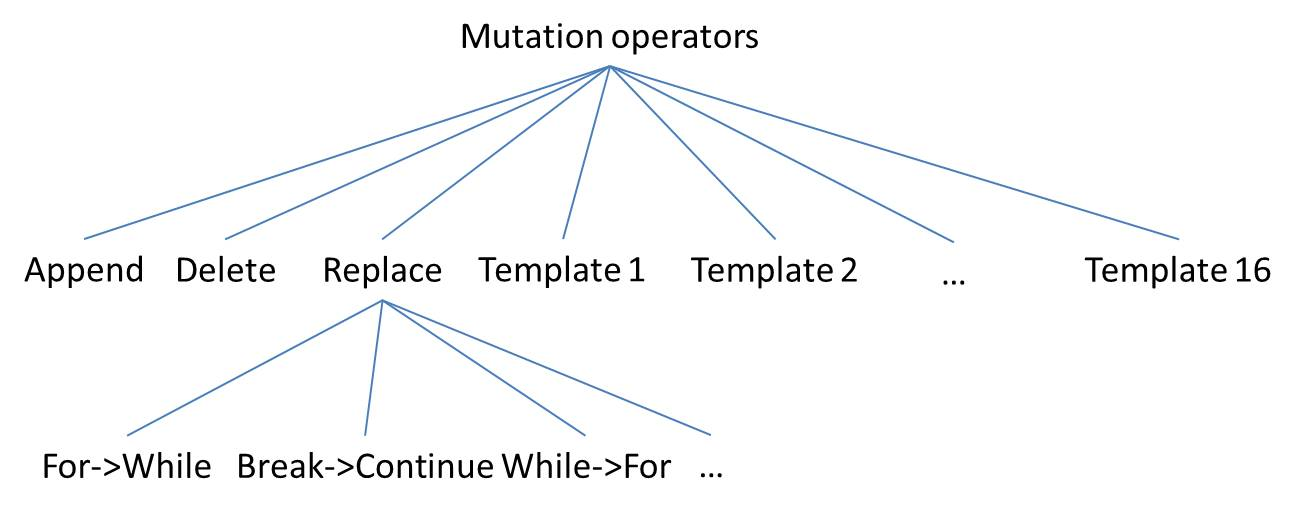
\includegraphics[scale=0.4]{Picture2}
%  \caption{Two level probabilistic model}
%  \label{fig:probModel}
%\end{figure}

We extend an open-source implementation of the GenProg technique adapted for Java
by implementing the mutation operators from
Section~\ref{categorization} as well as a mechanism that allows the tool to
select between the mutation operators according to the probabilities described by
a given model. %\footnote{https://bitbucket.org/clegoues/genprog4java}  
We construct a two-level model that effectively counts incidences of all considered
mutation operators, and fix code used in replacements. The two-level probabilistic model generalizes previous work proposing a replacement-only model~\cite{Soto16}:

\subsubsection{Mutation operator probabilistic model}
The \textit{Mutation operator probabilistic model} 
describes the probabilities of choosing between the several different mutation 
operators at a particular fault location.
%
To build the \textit{Mutation operator probabilistic model} 
we count the number of incidences of each mutation operator observed in our
dataset, matched as described in Section~\ref{sec:mining}. Mutation operator probability is then
weighted by its appearance in the dataset.  

For repair of a given statement, we consider only the mutation operators applicable (e.g. we can not apply \emph{Parameter replacer} to a \emph{BreakStatement}).

In our dataset overall, the Template-Based mutations comprise 29.26\% of the corpus; Statement-Edit mutations make up 70.74\% of the 
corpus.

\subsubsection{Replacements probabilistic model}
If the ``Replacement" mutation operator is 
selected, the \textit{Replacements probabilistic model} describes the probability of replacing one statement (``replacee") with
another (``replacer"), thus informing the selection of replacement fix code.
%\footnote{https://goo.gl/mMFbnQ
We consider 
the 22 different types detailed by the Eclipse
JDT\footnote{AssertStatement, Block, BreakStatement, ConstructorInvocation, ContinueStatement, DoStatement, EmptyStatement, EnhancedForStatement, ExpressionStatement, ForStatement, IfStatement, LabeledStatement, ReturnStatement, SuperConstructorInvocation, SwitchCase, SwitchStatement, SynchronizedStatement, ThrowStatement, TryStatement, TypeDeclarationStatement, VariableDeclarationStatement, WhileStatement \label{stmtNames}} as
direct known subclasses of the class \texttt{Statement}, and the incidence with which
each 
replaces another. For example: ``What is the observed incidence of a \texttt{For} loop 
replacing a \texttt{While} loop?" Given 22 statement types, any of which may replace one
another, there are 484 possible combinations. 
Note that the observed probabilities are not reciprocal, e.g. 
that the probability of a \texttt{For} loop replacing a \texttt{While} loop is different from the 
probability of a \texttt{While} loop replacing a \texttt{For} loop.
This model is built analogously to the
mutation operator model, based on replacer/replacee statement incidence. 

To build both models we perform an incidence count of each mutation operator and replacement observed in our
dataset, matched as described in Section~\ref{sec:mining}, and then apply Laplace smoothing~\cite{Russell10} with $\alpha$ = 1 to account for 0 occurrences.

\subsection{Multiple edit association rule mining} 
\label{multEdit}

Although such single-edit patches can be
sufficient to repair non-trivial bugs in real software, the majority of bug fixes in real
software require multiple edits~\cite{zhong15,Soto16}. The combination of possible mutation
 operators to apply in a sequence increases exponentially as we add more source
 code changes, motivating a more precise mechanism to navigate the vast search
 space. 

As a first step towards mitigating this limitation, we propose 
an initial analysis of multi-edit 
source code changes by mining a more expressive model of common changes. In
particular, we extract \emph{association rules} between single edits 
to model chains of single edit changes, capturing the way humans create these kinds of fixes.

Association rules are if/then statements that show relationships between elements in a dataset which happen frequently together. We use the 
well-known association rule mining algorithm
Apriori~\cite{Agrawal94}, which identifies frequent 
individual items in sets of transactions (commits, in our context).  We extend these sets into 
larger sets that appear often in the transactions. We mine association rules from each of the models described in Section~\ref{armRes} by transforming each of the mutation operator count and replacement count from 
each of the commits studied into a \emph{transaction} to be analyzed. 

Two other basic concepts critical to the Apriori method are \emph{Confidence} and \emph{Support}.
Formally, we define Confidence as:

\begin{center}
$conf(X \implies Y) = \dfrac{supp(X \cup Y)}{supp(X)}$ 
\end{center}

Where X and Y are possible items in a transaction (mutation operators and replacements in our
context for the Mutation operator probabilistic model and the Replacements probabilistic model accordingly). Confidence is calculated according to its Support (\emph{supp}), 
an indication of how frequently the set of mutation operators or replacements (itemset) 
 occurs in the transaction base.
Formally:

\begin{center}
$supp(X) = \dfrac{|\{t \in T; X \subseteq t\}|}{|T|}$
\end{center}

Where X is the itemset and \emph{t} is each individual transaction in
the database of transactions \emph{T}. Apriori identifies the frequent mutation
operators and replacements that happen together, iteratively extending them to larger
itemsets that appear often in the transactions as identified by these metrics.

To create these association rules among several mutation operators, we mine the
transactions made out of the commits created by humans in the corpus of projects
studied and we look for rules that have at least 90\% Confidence, where
Confidence is an indication of how often the rule has been found to be true.


\section{Evaluation} \label{evaluation}

We evaluate our model both independently and as part of an automatic repair
technique.  We first evaluate the predictive power of the model by analyzing the
number of correctly predicted mutation operators across a large dataset, using 10 fold cross
validation to mitigate and assess the risk of overfitting
(Section~\ref{sec:generalize}). We evaluate our new APR approach on 18 \todo{ change this number if we get more results} different bugs from the Defects4j platform (Section~\ref{repResults}) both in terms of speed, measured in the number of variants it takes to find a patch, and quality, by comparing against the patches created for these same bugs by other state-of-the-art repair techniques.  Finally, we present the most common 
association rules between mutation operators in our corpus
(Section~\ref{armRes}). 

%We also include a section for 
%discussion(Section~\ref{discussion}) and threats to validity (Section~\ref{threatsVal}) 



\subsection{Experimental setup}
All experiments are performed on a server 
consisting of 16 processors Intel(R) Xeon(R) CPU E5-2699 v3, with 2.30 GHz each
processor, 46080 KB cache each, and 32 GB RAM memory, operating system Ubuntu 
14.04.5 LTS.



\begin{figure}[ht]
\centering

\begin{tabular}{lllll}
\toprule
           &   Project  &             &   &  Defects\\
Identifier &    name & Description & Test cases & considered \\
\midrule
Chart & JFreechart & Java chart library & 2205 & 3\\
Closure	& Closure compiler	 & JavaScript handling tool & 7927 & 4\\
Lang	& Apache commons-lang & String manipulation classes  & 2245 & 4\\
Math	& Apache commons-math & Mathematics components for Java & 3602 & 4\\
Mockito &	Mockito	 & Mocking framework for junit tests & \todo{I can't find this data} & 0 \\
Time	& Joda-Time & Date and time classes  & 4130 & 3\\
\bottomrule
\end{tabular}
\center
  \caption{Description of projects that comprise Defects4j \todo{re visit the number in the last column to see if we have found a new patch}}
  \label{defects4j}
\end{figure} 

We consider a subset of the Defects4j~\cite{just14}
benchmark, a database and extensible 
framework of real bugs that enables reproducible studies in software testing 
research. This database currently contains 395 real bugs from six
open source programs shown in Figure~\ref{defects4j}, along with developer-provided test suites, cases that
expose each bug,  and
corresponding developer-provided patches.\footnote{Note that we initiated this study when Defects4J
  contained five subjects, and thus have no bug instances from the recently-added
  Mockito project.} Defects4j has been previously used
in evaluating previous work in APR~\cite{Durieux15}.
In keeping with APR's typical focus on smaller patches, we
restrict attention to the first bugs from each project that required a 
single line edit.
To diminish the degree of randomness in this experiment and control for the
effect of the mutation probabilities specifically rather than inefficiency and noise
in fault localization,  we manually
set fault localization for each bug. Anecdotally, we observe that less-accurate fault localization increases the amount of
time taken to repair these defects, but does not decrease expressive power. 

When running this experiment, we set the size for each population to 40 for consistency with 
previous work~\cite{legoues12,kim2013}, ran 20
seeds per trial, 10 generations, a timeout of 4 hours for each run, in keeping with 
recommendations on the assessment of stochastic techniques~\cite{arcuri11}.

To compare the efficacy of different types of mutation operators,
we tested three operation sets: (1) Statement-Edit mutations only (2) Template-based mutations 
only (3) All mutations.  We average (the number of variants necessary to create a repair) overall seeds. We use number of variants as a measure for speed since it is a machine- and test suite-independent proxy for time.

As a proxy for patch quality (to
mitigate the risk of plausible but as yet incorrect patches~\cite{Qi15}), we
evaluate patches using a held-out test suite~\cite{legoues2012,smith15} by automatically building a second
test suite that independently describes the same behavior as the test suite that
guides the search process. 

Figure~\ref{heldOut} describes the specifics of the held out test suites. We use Randoop~\cite{pacheco07}, an established
automatic test suite generation tool for Java, to generate this second test
suite. We run Randoop with a ten minute budget (six times the default value) to create the held-out test suites. We also use Cobertura\footnote{http://cobertura.github.io/cobertura/} to calculate the coverage of the test suite over the class that contains the human fix. 

\begin{figure}[]
\centering
\begin{tabular}{llll}
\toprule
         &             & \multicolumn{2}{c}{Coverage} \\
Project & \# tests & Line & Condition \\
\midrule
Chart 1 & 4285 & 32.9\% & 24.0\% \\
Closure 10 & 1493 & 5.5\% & 3.0\% \\
Closure 18 & 1615 & 32.1\% & 17.6\% \\
Math 2 & 6933 & 100\% & 100\% \\
Time 19 & 3650 & 75.4\% & 58.0\% \\
\bottomrule
\end{tabular}
\caption{Held-out test suite data; suites created using Randoop, with a budget
  of 10 minutes. Coverage is evaluated using Cobertura.}
\label{heldOut}
\end{figure}    


\subsection{Model generalization}
\label{sec:generalize}
  

%\begin{figure}[ht]
%\tabcolsep=0.18cm
%\begin{tabular}{llllllllllllllllllllll}
%\hline
%As & Bl & Br & Cl & Co & Do & Em & EF & Ex & Fo & If \\
%0\%&2\%&0\%&2\%&5\%&0\%&0\%&0\%&43\%&0\%&22\% \\
%\hline 
%La & Re & SC & Ca & Sw & Sy & Th & Tr & TD & VD & Wh \\
%0\%&0\%&2\%&2\%&0\%&0\%&3\%&2\%&0\%&19\%&0\% \\
%\hline
%\end{tabular}
%\\
%\caption{Example of the Return Statement row of a sub-model created from 
%the training data. Replacee probabillities of the replacer ReturnStatement. The acronyms represent the statement kinds detailed in footnote \ref{stmtNames} \todo{The notes said to remove this, but we can't explain the following section without it, so I am keeping it for now}}
% \label{fig:exPredReturn} 
%\end{figure} 

In this section we want to evaluate the consistency of the corpus and provide internal validity to our results by performing a 10 fold cross validation over our model. We built the model with the 500
projects in Github with the most stars.
 This is to generate the largest code base so far to the best 
of our knowledge, surpassing all the previous state of the 
art~\cite{long16proph,Soto16,zhong15,martinez15,xuan16}. 
In these experiments, we include all mutations described in
Section~\ref{categorization}.

First, we evaluate the predictive power of our 
replacements model. Our high-level research question concerns whether 
our mined models are likely to identify the correct fix code across a large
dataset, suggesting its potential utility in a repair context.  To this end, we
compare its predictive accuracy to an \emph{equally distributed} model, in which
the probability of selecting any replacee statement is uniformly random. 
We assess the degree to which each model correctly predicts the
replacer statement for given replacee statements, within the top 5 produced
choices. Perfect accuracy (correctness in the Top-1 most likely choice) is unnecessary, since automatic program repair approaches iterate through several different candidate patches until finding the appropriate fix;
however, the noisy search problem suggests that a relatively tight bound (top-5)
is likely appropriate.  Additionally, we found observationally that the top-5
choices serves as a point of inflection between the mined and equal model
performance. 

We use 
10-fold cross validation~\cite{kohavi95} to mitigate and assess the risk of overfitting and avoid testing and training on
the same data. 
We segregated the projects in our corpus into 10 
random folds. For each 
fold, we use one fold for testing, and the remaining nine for training. We aggregate the results over all 10 folds counting the number of testing instances that are correctly predicted 
by the first five guesses from the training sub-model.   

To illustrate, consider a simple example. Assume the following
simple bug-fixing patch from our corpus: 

\begin{lstlisting}[frame=single]
+ if(i > l.size()) {
    return l.get(i); @//original faulty location@
+  }    
\end{lstlisting}

The developer has replaced the original \texttt{return} with an
\texttt{if-then} statement that wraps it.  Our goal in assessing our model is,
assuming the selected mutation operator 
is \emph{replace}, how often will an \emph{IfStatement} be predicted as the
replacer? If it is returned in the first five instances in a model, the model
correctly predicts this instance. We aggregate correctly predicted instances over all folds.

Each trained model describes the dataset via
a distribution identifying the (normalized) frequency with which each statement is replaced 
by another. Each combination is described by 
$E_{n,m}$, 
where \emph{n} is the statement being replaced (replacee) and \emph{m} the statement it is 
replaced by (replacer).  A predictive model $TP_{n,m}$, $\forall n,m: 1<=n<=22 \land 1<=m<=22$, 
describes how often each statement is replaced by 
other kinds of statements. 

%For example, if the approach picks at random the statements: Assert Statement 
%$TE_{13,1}$, 
%Do Statement $TE_{13,6}$, Expression Statement $TE_{13,9}$, Throw Statement 
%$TE_{13,18}$ and Try Statement $TE_{13,19}$. Then we 
%would match how many of the instances in the testing data were correctly 
%predicted by this equally distributed schema.

%In this example, the 4 instances of Expression Statement $E_{13,9} = 4$, the 
%instance of Do 
%Statement  $E_{13,6} = 1$, and the instance of Try Statement $E_{13,19} = 1$ 
%would be considered to be correctly 
%predicted; while the 2 instances of If Statement $E_{13,11} = 2$, and the 2 
%instances of 
%Continue Statement $E_{13,5} = 2$ would be considered to be incorrectly 
%predicted. Since the 
%equally distributed approach in this example correctly guessed 6 out of 10 
%instances of the testing data, we would then say that in this particular case, 
%the equally distributed approach correctly predicted 60\% of the instances in 
%the testing set.  


\begin{figure}[ht]
{\footnotesize
{\centering
\begin{tabular}{l|rrr|rrr}
\toprule
   &\multicolumn{3}{c|}{Replacements} &\multicolumn{3}{c}{Mutations} \\
\midrule
Fold	& \# &Prob& EqDist& \#&Prob& EqDist \\
\midrule
1	& 155&70\%&	25\% &17313&  95\% & 64\%   \\
2	& 86&100\%&	25\%  & 17232& 93\% & 63\%   \\
3	& 81&82\%	&23\%  & 16754& 95\% & 81\% \\
4	& 101&81\%	&40\%  & 14159& 94\% & 9\%   \\
5	& 99&90\%	&27\%  & 17022& 95\% & 2\%  \\
6	& 75&84\%	&21\%  & 14945& 95\%& 58\%  \\
7	& 79&86\%	&24\%  & 12901& 93\%& 7\%  \\
8	& 55&96\%	&23\%  & 10552& 95\%& 27\%  \\
9	& 82&88\%	&8\%  & 14568& 93\%& 62\% \\
10	& 116&100\%	&31\% & 19140 & 95\% & 6\% \\
\midrule
Mean	& 192.9 &87.7	&24.7& 15458.6  & 94.3 & 37.9  \\
\midrule
Std dev	& 320.23&9.33&	8.01 & 2530.27 & 0.94 & 30.49   \\
\midrule
Sum & 1929&877 & 247 &  154586& 943 & 379  \\
\bottomrule

\newline
\end{tabular}
\center
  \caption{Correctly predicted edits, across 10 folds of data.
The replacement probabilistic model (left) predicts
    the correct replacement statement 87\% of the time,
    an improvement of almost a factor of 4 over the equally-distributed model. 
    The mutations model (right) outperforms the equally-distributed model by 
    almost a factor of 3. The \# columns show raw instance count per fold. \label{results10fcv}} 
}}

\end{figure} 


%\begin{figure}[!h]
%  \centering
%    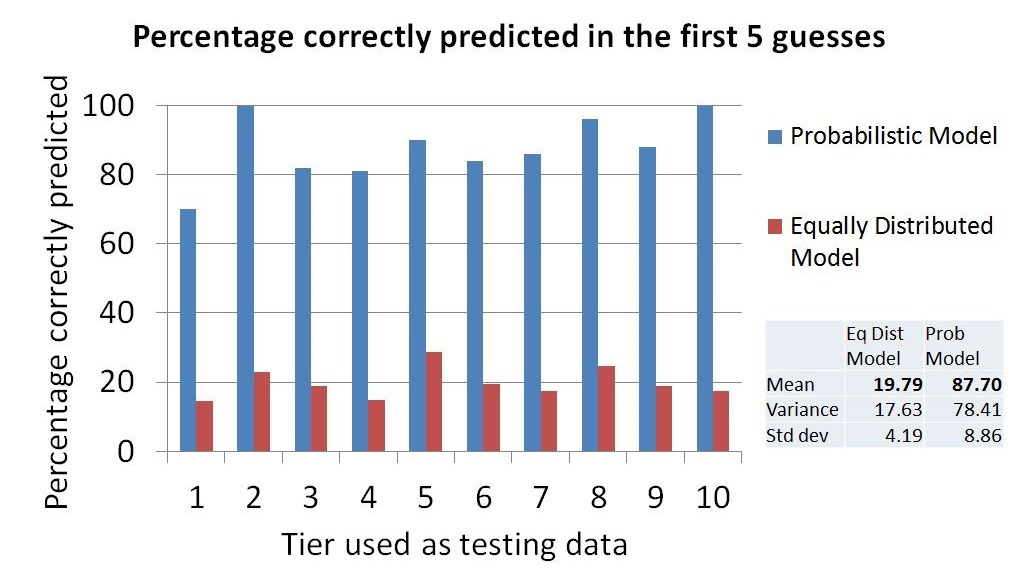
\includegraphics[scale=0.33]{sanity1}
%  \caption{   }
%\end{figure}
Results are shown in Figure~\ref{results10fcv}. For each fold, we show the instance count and percentage of correctly 
predicted instances within the top five
guesses of both the equally distributed and the replacements model. The
third and fourth columns show the percentage of correctly predicted
instances using the top five  
guesses of the sub-model of each of the folds for the replacements model. The sixth and seventh columns are percentage of correctly predicted instances for the mutations model. Columns two and five show
the number of instances in each of the folds. We have a difference of 63\% between the means of the two models in the replacements model, and a difference of 56.4\% between the mean values of correctly predicted instances in the probabilistic and equally distributed models for the mutations model. \todo{a)is it statistically significant?} We can infer from the data presented that the use of a probabilistic model is beneficial to find the correct mutation operator to patch a bug faster and with higher accuracy. We can also infer that when using the probabilistic model the search space is built in an informed manner, therefore the probabilities of obtaining the correct patch are higher due to the fact that this approach doesn't have to blindly look in all the search space as the equally distributed approach.


\subsection{Single line bug repair}
\label{sec:single}

\begin{figure*}\centering
\begin{tabular}{r|rr|rr|rr|rr|rr|rr}
\hline
 &\multicolumn{4}{c|}{Statement-Edit Only} & \multicolumn{4}{c|}{Template-based Only} & \multicolumn{4}{c}{All Mutations} \\ 
  \hline
 & \multicolumn{2}{c|}{Equally Dist} & \multicolumn{2}{c|}{Probabilistic} & \multicolumn{2}{c|}{Equally Dist} & \multicolumn{2}{c|}{Probabilistic} & \multicolumn{2}{c|}{Equally Dist} & 
 \multicolumn{2}{c}{Probabilistic} \\
\hline
Bug Name & Time & Quality &  Time & Quality &  Time & Quality&  Time & Quality&  Time & Quality&  Time & Quality \\
  \hline
 
  Closure \#10 & {221.0}& {100\%} & {179.5} &{100\%} & {175.1}&{100\%} & {121.3}&{100\%} & {163.3}&{100\%} & {157.4}&{100\%} \\

 Closure \#18 & \multicolumn{2}{c|}{Not found} & \multicolumn{2}{c|}{Not found} & {36.2}&{100\%} & {197.5}&{100\%} & {45.0}&{100\%} & {139.0}&{100\%} \\

Math \#2 & \multicolumn{2}{c|}{Not found} & \multicolumn{2}{c|}{Not found} & {109.4}&{0\%} & {39.6}&{0\%} & {109.4}&{0\%} & {39.6}&{0\%} \\

 Time \#19 & {94.1}&{100\%} & {80.7}&{100\%} & \multicolumn{2}{c|}{Not found} & \multicolumn{2}{c|}{Not found} & {135.1}&{100\%} & {91.9}&{100\%} \\

 Chart \#1 & {1.8}&{0\%} & {7.3}&{0\%} & {4.9}&{0\%} & {19.0}&{0\%} & {2.2}&{0\%} & {4.8}&{0\%} \\
\hline

\end{tabular}
\newline
\center
		\caption{Repair success of various models for three different operator
          sets.  For each, we report time in terms of variants evaluated to a
          repair, and quality as the percentage of patches created for that bug that pass the held-out test suite. \label{tab:singleLineBugs}}

\end{figure*}

In this subsection, we compare the performance of an
automatic program repair tool using the probabilistic model to one using the
equally distributed model.  


\subsubsection{Repair results}   \label{repResults}
\todo{re visit this paragraph after we have the latest results}Our modified APR technique patched 5 of the 18 bugs, as shown in 
Figure~\ref{tab:singleLineBugs}. In the first row of Figure~\ref{tab:singleLineBugs} (Closure \#10) we can see
that in all three comparisons (Statement-Edit Only, Template-Based Only, and All
mutations), the probabilisitc model outperforms
the equally distributed model. This happens as well for
Math \#2 and Time \#19 except for the cases where no patch was
found. By contrast, for bugs Chart \#1 and Closure \#18, the equally
distributed approach finds a patch faster on average. This is due to the fact
that these bugs are patched with mutations that are rarely to applied by developers (Expression Replace, and Replacement accordingly),
therefore it is more likely that the mutation operator will be chosen by randomness
than by the developer-informed model.

Our results also show that considering all available mutation operators is
preferable to 
restricting the mutation operator pool to just one of the categories \todo{revisit this after we have more results}. For the
Statement-Edit category: 3 out of 6 were fixed faster when combining it with
Template-Based mutations, and 3 out of 6 were slower. For the Template-Based
category: 4 out of 8 were fixed faster when combining it with Statemtent-Edit
mutations, 2 out of 8 were the same, and 2 out of 8 were slower. This suggests
that the expressive power afforded by an increased set of operators may
outweight the commensurate increase in search space size, though it is safe to
assume that this benefit must be supported by sufficiently accurate fault
localization. 

 %\footnote{\url{https://github.com/mausotog/ReplacementsEmpiricalStudy/tree/master/Randoop10MinHeldOutTestSuites}} 
We noticed a
constant behavior regarding the different sets of mutations. In this sample, if
a model is able to find a patch faster, this appears independent of the mutation
set.  We also notice that
the quality of patches produced  appears constant, and unaffected by model:
either the tool produces patches in 
that all pass the second test suite, or it produces patches that do not. 
%\subsection{Bugs fixed with a multi line edit within a function}
%Last evaluation with the bugs we found had a fix

\subsubsection{Repair example} \label{examPatches}

\begin{figure}[t]
\begin{lstlisting}[frame=single]
LegendItemCollection result = 
  new LegendItemCollection();
if (this.plot == null) {
  return result;
}
int index=this.plot.getIndexOf(this);
CategoryDataset dataset = 
  this.plot.getDataset(index);
@ -if (dataset != null) {
  - return result;
  -}@
int seriesCount=dataset.getRowCount();
	\end{lstlisting}

\begin{lstlisting}[frame=single]
LegendItemCollection result = 
  new LegendItemCollection();
if (this.plot == null) {
  return result;
}
int index=this.plot.getIndexOf(this);
CategoryDataset dataset = 
  this.plot.getDataset(index); @
 + if (dataset != null) { 
 + this.itemLabelGeneratorList=new ObjectList();
 + this.toolTipGeneratorList=new ObjectList();
 + this.urlGeneratorList=new ObjectList();
 + this.legendItemLabelGenerator = 
 +  new StandardCategorySeriesLabelGenerator();
 + this.backgroundAnnotations=new ArrayList();
 + this.foregroundAnnotations=new ArrayList();
 + }@
int seriesCount=dataset.getRowCount();
	\end{lstlisting}
	\caption{Top: A snippet of the source code of the Chart 1 bug fixed using the
      probabilistic model, with a deletion similar to the developer
      patch. Bottom: the same bug, fixed using the equally distributed
      model by 
      allocating global variables that may be used later, much unlike the human
      patch.\todo{Mau, please have these listings numbers start at a number
        like the one where it starts in the actual code.}\label{fig:chart1.3}}
\end{figure}


In this subsection, we provide example patches produced using the alternative
models, as compared to a human patch.  Consider the snippet of code corresponding
to the first Chart bug (and its developer fix) from the Defects4J dataset
(Figure~\ref{fig:chart1.1}, top).  The developer patches this bug by deleting the if
statement.  The mined statement-level mutation model favors deletion, and thus
our repair efforts found patches that removed either the entire \texttt{IfStatement}, or only its body (line 9).
By contrast, the equally-distributed model has a higher probability of leading
to a patch such as the one shown in the bottom of Figure~\ref{fig:chart1.1}.  This test case
passes when, in the case that \texttt{dataset} is not null, nothing is returned;
this patch avoids this, but also allocates state variables that are not
necessary at present (and whose state may have unknown effects in other
executions). 

\subsection{Comparison against state of the art approaches}

 \begin{figure*}
\centering
\begin{tabular}{l|l|ll|ll|ll|ll|ll}
\toprule
& Number of test cases & Probabilistic Model & NFTC & GenProg & NFTC & TRP & NFTC & PAR & NFTC & Nopol  & NFTC  \\
\midrule
Closure 10 &1493 & SequenceExchange & 0 & No patch & No patch & No patch & No patch & No patch & No patch & Found & 28   \\
 & & SequenceExchange & 0 & No patch & No patch & No patch &No patch  & No patch & No patch & No patch & No patch   \\
\midrule
Closure 18 & 1615 & ExpRemove & 0  & No patch & No patch & No patch & No patch & No patch & No patch &Found &  1  \\
\midrule
Math 2 & 6933 & MethodReplace & 170 & No patch & No patch & No patch & No patch & MetthodReplace & 170 & Found & 0  \\
\midrule
Time 19 & 3650  & Append & 0 & Append & 188 & Append & 188 & No patch & No patch & Found &  188 \\
 & & Replace & 0 & No patch & No patch & No patch & No patch & No patch & No patch & No patch & No patch \\
\midrule
Chart 1 &  4285 & SequenceExchange & 1 & Replace & 1  & Delete & 1 & ExpAdd & 1 & No patch &   \\
 & & Delete & 1 & Delete & 1 & Replace &1  & ExpReplace & 1 & No patch & No patch   \\
 && Delete & 1 & Replace & 1 & Delete & 1 &  No patch& No patch& No patch & No patch  \\
 && SequenceExchange & 1 & Delete & 1 & Delete &1  & No patch & No patch & No patch & No patch   \\
 & & ExpReplace & 1 & Delete & 1 &No patch & No patch & No patch & No patch & No patch & No patch   \\
 & & No patch & No patch & Replace & 1 & No patch & No patch & No patch & No patch & No patch & No patch  \\
 \bottomrule
\end{tabular}
  \caption{Quality assessment between the probabilistic model-based repair and
    other state of the art approaches. The NFTC column shows Number of Failed
    Test Cases, for each patch, evaluated against the held-out test suite.  NFTC
    of 0 means the patch fully generalized to the the held-out test
    suite.\todo{mau, please fix this as discussed on Monday so that the column
      headers make sense, and then I'll make the figure fit.} \label{stateOfTheArtComparison}} 
\end{figure*}


\begin{figure}[t]
\begin{lstlisting}[frame=single]
boolean staleInputs = false;
@-if(options.dependencyOptions.needsManagement() && options.closurePass){
+if(options.dependencyOptions.needsManagement()){
@  for (CompilerInput input : inputs) {
    // Forward-declare all the provided types, so that they
    // are not flagged even if they are dropped from the process.
    for (String provide : input.getProvides()) {
      getTypeRegistry().forwardDeclareType(provide);
    }  
  }
	\end{lstlisting}


\begin{lstlisting}[frame=single]
boolean staleInputs = false;
@-if(options.dependencyOptions.needsManagement() && options.closurePass){
+if (com.google.javascript.rhino.Node.this.type <= com.google.javascript.rhino.Node.IS_DISPATCHER) {
@  for (CompilerInput input : inputs) {
    // Forward-declare all the provided types, so that they
    // are not flagged even if they are dropped from the process.
    for (String provide : input.getProvides()) {
      getTypeRegistry().forwardDeclareType(provide);
    }  
  }
	\end{lstlisting}

	\caption{Top: A snippet of the source code of the Closure 18 bug as fixed using the
      probabilistic model, identically to the developer patch. None of the other
      approaches found an identical patch.  Bottom: the Nopol fix for the
      Closure 18 bug, which does not generalize to a held-out test
      suite.\label{closure18prob}\todo{Mau, please have the lstings start the
        numbering at the line number of the actual sourcecode in question
        (rather than at 1)}}
\end{figure}

In this section we compare the patches produced by our approach, using all the
mutation operations and the probabilistic model, against
four previously-proposed tools:  GenProg, TrpAutoRepair, PAR and Nopol.\todo{add
  a reference for each of these.}

We extend an available open-source implementation of GenProg adapted for Java to
include the behavior and mutation operators of these first three approaches,
since they were originally built to target C (GenProg and TRPAutoRepair), or
have not made their code available (PAR). We also compare our approach to
Nopol~\cite{xuanNopol}, an automatic repair tool of conditional statement for
Java programs. The authors have created patches for the same benchmark used in
this study~\cite{martinez2016} and made their results publicly
available.\footnote{https://github.com/Spirals-Team/defects4j-repair/tree/master/results/2017-march}
For the comparison with Nopol we have used the more up-to-date dataset available
in their website marked as ``March 2017".\todo{pending to add more justification
  depending on Martin's response} 
In this study we do not compare directly to SPR/Prophet~\cite{long16proph}
mutation operators because they use machine learning to tune the probabilities
to pick their schemas and is thus much harder to re implement
faithfully. \todo{this thought makes more sense in related work.}

Figure~\ref{stateOfTheArtComparison} shows results, including, for each patch,
the number of held-out tests the patched program fails. Of the \todo{how many?}
patches created by our approach, 
five pass all held-out test suite (45.5\%). None of the GenProg,
TRPAutorRepair, or PAR patches fully generalize; 25\% of Nopol's patches do.
This gives us confidence that our approach produces high
quality patches in comparison with the alternatives created by state-of-the-art
tools. 

One example demonstrating the quality improvement afforded by the probabilistic
model-based approach is evident for the Clousre 18 bug.  in which we can very clearly see the success of our approach when
applying the probabilistic model is Closure 18 as seen in
Figure~\ref{closure18prob} where, not only did our approach created the exact
same patch as the human did, but also our approach was able to find the patch
within the time frame specified before the execution is shutdown by one of the
constraints per execution while other approaches that are able to create this
patch, couldn't because they ran out of time.

This example was fixed by the human by removing an expression from an
\emph{IfStatement} as seen at the top of Figure~\ref{closure18prob}. 
Although PAR includes this a mutation operator for this task, its uniform
weighting scheme appears less efficient than our probabilistic model. Nopol was
able to create a patch for this example as shown at the bottom of 
Figure~\ref{closure18prob}, but this patch is not able to generalize to a
held-out test suite.

\subsection{Association Rule Mining} \label{armRes}

We mined our corpus using the Association Rule Mining algorithm Apriori 
to find rules of mutation operators and 
replacements that commonly happen together providing an intuition regarding
how to form multi-edit
source code changes.

\paragraph{Mutation operator rules}
We mine rules from our corpus as described in Section~\ref{multEdit}.  
These rules are ranked by their confidence. In this case, the top 10 \todo{we can shorten this to 5 rules if we need space} rules shown
below have a confidence of 100\%, meaning that in 100\% of the cases
studied, every transaction that showed the antecedent also showed the consequent.
They are obtained with a 1\% support, which means that each of these rules
individually appear in at least 1\% of all the transactions in the
corpus. We show the top association rules for the mining of single edit 
mutation operators to indicate the structure of the rules; and release the full set of mined
rules with over 90\% Confidence and 0.1\% Support:\footnote{We will release the full list of mutation operator and replacements rules post blind-review.} %\footnote{\url{https://github.com/mausotog/ReplacementsEmpiricalStudy/blob/master/ResultsAssociationRuleMiningMutOperators.txt}} 

%Minimum support: 0 (1 instances)
%Minimum metric <confidence>: 0.9
%Number of cycles performed: 20

\begin{itemize}
\item Replace \& Delete $\implies$ Append
\item Delete \& AddNullCheck $\implies$ Append
\item Replace \& SeqExchanger $\implies$ Append
\item Replace \& ParamReplacer $\implies$ Append
\item Delete \& CasteeMutator $\implies$ Append
\item Replace \& Delete \& ParamReplacer $\implies$ Append
\item Replace \& AddNullCheck $\implies$ Append
\item Replace \& Delete \& SeqExchanger $\implies$ Append
\item Delete \& ExpressionAdder $\implies$ Append
\item Delete \& AddNullCheck \& ParamReplacer $\implies$ Append
\end{itemize}

Append is the most common single edit mutation operator applied by developers. This behavior is
reflected in the fact that it is the consequent in the all the top mined
rules.  

\paragraph {Replacement rules} We also analyzed association rules for the
replacements model, obtaining
the following rules with a 0.01\% Support and 90\% Confidence. %\footnote{\url{https://github.com/mausotog/ReplacementsEmpiricalStudy/blob/master/ResultsAssociationRuleMiningReplacements.txt}} 
The best rules we found are: \todo{we can shorten this to 5 if necessary}
%Minimum support: 0.0001 (1 instances)
%Minimum metric <confidence>: 0.9
%Number of cycles performed: 20
\begin{itemize}
\item Block replaces ReturnStatement \& ExpressionStatement replaces IfStatement $\implies$ Block replaces IfStatement
\item VariableDeclarationStatement replaces AssertStatement $\implies$ SwitchCase replaces BreakStatement
\item EnhancedForStatement replaces TryStatement $\implies$ ExpressionStatement replaces ReturnStatement
\item ForStatement replaces TryStatement $\implies$ ExpressionStatement replaces VariableDeclarationStatement
\item VariableDeclarationStatement replaces EnhancedForStatement $\implies$ ExpressionStatement replaces VariableDeclarationStatement
\item VariableDeclarationStatement replaces ForStatement $\implies$ ExpressionStatement replaces VariableDeclarationStatement
\item ForStatement replaces TryStatement $\implies$ IfStatement replaces TryStatement
\item VariableDeclarationStatement replaces ForStatement $\implies$ ForStatement replaces TryStatement
\item ForStatement replaces TryStatement $\implies$ VariableDeclarationStatement replaces ForStatement
\item VariableDeclarationStatement replaces ForStatement $\implies$ IfStatement replaces TryStatement
\end{itemize}

%Similar to the one described above, the authors have made available the full list of association rules with over 90\% Confidence and 0.01\% Support.\footnote{https://goo.gl/omk60t}
%REPLACE FOR CAMERA READY: https://github.com/mausotog/ReplacementsEmpiricalStudy/blob/master/ResultsAssociationRuleMiningReplacements.txt

Association rules provide an intuition of which common patterns of behavior developers use. These rules tell us what edits happen frequently together, which will help us further understand multi-edit source code changes, an understudied area that covers the majority of real life patches.

\section{Threats to Validity} \label{threatsVal}

\noindent\textbf{Internal validity:}
Regarding possible errors in our implementation and experiments, to run our
comparison with Genprog, we used an open-source implementation of GenProg
targeting Java. We release our code, as well as our templates,
independently-generated tests, and mined models for scrutiny and extension by other
researchers, to mitigate the risk of errors in our implementation or approach. 
 We also use 10-fold cross validation in
assessing our model, to reduce the risk of training and testing on the same
data.  
%REMOVE THIS FOR CAMERA READY
%in the project mentioned before 

\noindent\textbf{External validity:} 
It is possible 
that our results will not generalize to external datasets and to
real bugs. To mitigate this concern, we build our model from well-known open-source
programs, covering a diversity of applications, and distinct from the dataset
from which the models were mined, and we evaluate our approach with bugs from an open-source framework.

There is also risk of producing low quality patches that would not 
generalize
to a different description of desired program behavior. We attenuate 
this by 
assessing the quality of the generated patches with a held-out test suite.
There is risk in the fact that we are manually giving the
faulty location to the APR tool, since APR tools do not know in advance what the 
fault location is. This is for the purposes of evaluating the patch creating 
process
only without the noise that fault localization might introduce.

\noindent\textbf{Construct validity:}
Regarding the suitability of our evaluation metrics, we evaluate patch
quality by running the generated patches on a second test suite created
from a human patch, which is to a certain extent a biased measure since we can
not guarantee that the human created patch is perfect~\cite{smith15}. Nevertheless, we consider 
this to be a
best known practice, since this way we provide an alternative to subjectively 
asking a biased human developer
whether he/she considered the patch to be correct or not. 

We also rely on Randoop~\cite{pacheco07} as our test suite generation mechanism 
for the held-out test suite used for evaluation, and we acknowledge that the 
test suites created by this tool may not be perfect, nor provide full coverage. 
Nonetheless, this is a state of the art test suite generation tool that mitigates the risk of bias in manually constructing evaluation test suites.

\section{Related Work} \label{relatedWork}

There have been previous efforts to create a model based on human behavior.  
Soto et al.~\cite{Soto16} 
built a probabilistic model to describe the replace 
operator only. They do not evaluate the model in the context of a repair
tool, and the model is based on an instance count of statements rather than an a more 
accurate analysis of AST differences, which our model was built from.  
HDRepair~\cite{xuan16} 
uses fix history
to help assess patch suitability and fitness in the context of a genetic
programming search strategy. The fitness of the generated
fix candidates is determined by the frequency with which the changes included in
a given patch occur in the corpus, using a Graph-based representation of the bug
fixes.  Similarly, Prophet~\cite{long16proph} uses a
probabilistic model of a subset of our considered mutation operators built on 
the history of 8 different projects to rank candidate
patches.  Our approach follows this intuition to mimic human
behavior; unlike the previous work, we apply this knowledge when actually
creating patch candidates rather than when evaluating them, which reduces the 
search space at the time of creation.  

Zhong and Su~\cite{zhong15} perform an empirical study of
real bug fixes on six projects, studying the incidence of three mutation
operators, among other questions about the applicability of APR.  Martinez and
Monperrus~\cite{martinez15} similarly study mutation operator incidence across 
14 
projects. Our work considers a broader set of
mutation operators over a larger corpus, the largest, to the best of our
knowledge, studied in existing work. To counter the 
risk of overfitting to a small set of training projects as performed before, our 
current study trains the model over 500 projects, covering a diversity 
of domains.

Par~\cite{kim2013} describes a manual set of 10 templates of common behavior to
create patches, showing that such templates result in patches of higher
human-adjuded acceptability than statement-edit-based patches.  Our study takes 
into consideration a superset
of these templates, provides steps towards
accounting for multi-edit source code changes, an understudied problem, and,
importantly, mines and models these operators and their incidence automatically
(rather than manually).

There exist a broad array of APR techniques proposed, especially recently; we
survey many of them in Section~\ref{background}, focusing on heuristic or
syntactic generate-and-validate techniques.  Semantic-based techniques use
semantic analysis or reasoning~\cite{nguyen13,mechtaev15,Mechtaev2016}, or
semantic search~\cite{ke15} to construct candidate patches.  Similarly,
synthesis-based repair is a family of techniques that uses constraints to build
patches following the description of the constraints~\cite{jin11,wei10}. These constraints may be
specifications created by developers, formal verification, invariants,
etc.~\cite{jin11,wei10}.  Such techniques typically use synthesis to construct
repairs, with a different mechanism for both constructing and traversing the
search space, and our approach is thus less immediately comparable.
 

\section{Conclusion} \label{conclusion}

In this paper, we analyze the way in which current state of the art automatic 
program repair approaches select mutation operators to create candidate 
patches. We analyze, categorize and compare the mutation operators being used by 
state of the art approaches. We analyzed the last 100 bug fixing commits from 
the
500 most-starred Java projects on Github, which is the largest corpus analyzed
to date, to the best of our knowledge.  We created a two-level probabilistic 
model describing
the likelihood of selecting bug-fixing mutation operators, according to the
observed incidence of their use by human developers. All the data gathered, 
tools and test suites used in this study are publicly available for open peer review 
and scrutiny.

We evaluated our single-edit approach in several ways: by performing an internal 
evaluation of 
its predictive power (using 10 fold cross 
validation), by comparing the speed of the model by comparing it to an equally 
distributed model and  
 running them on 15 bugs using the database of bugs and extensible 
framework Defects4j, and finally by comparing the quality of the patches 
generated against patches created for these same bugs by other state of the art 
approaches. 

For these bugs, we measured the number of variants it takes to find the 
patch as well as the quality of produced patches, using a second 
automatically-created held-out test suite.
Note that in Figure~\ref{tab:singleLineBugs}, for the majority of bugs, the 
equally distributed model performed better than their equally distributed 
counterpart.
We also notice that applying different probabilities when constructing variants
does not make the patches found in either of the models more likely to pass a
second test suite for these five bugs. Further evaluation should be performed to
determine if one of the models creates higher quality patches than the other. 
Overall, however, we found that automatic program repair appears to benefit
from having a diverse mutation operator pool containing mutation operators from 
both categories,
rather than restricting their choices to just one category, increase in search
space size notwithstanding; future improvements in fault localization thus will
serve to further benefit from more precise models of mutation selection. 

Multi-edit source code changes are understudied, but cover
the vast majority of bug fixes in software systems. 
To move towards advancing this area, we constructed a set of association rules 
that describe 
how often different sets of mutation operators can predict the change that will 
come next, and how often subsets of mutation operators are applied together.

There is a tension between the Support and the Confidence measures in our 
transaction 
base, in which we 
evaluate the different mutation operators being applied to source code in bug 
fixing commits. 
If we increase the Confidence and decrease Support, we obtain rules such that
the antecedents and consequents have a higher rate of occurring together. By 
lowering Support this will produce rules that
do not occur often.  Although, when they \emph{are} selected, are very likely to 
be
correct. 

On the other hand, if 
we increase the Support and decrease the Confidence we would obtain rules that 
are guaranteed to happen in a certain percent of the corpus, which means,
the relationship described by the rules, happens often, but confidence is 
sacrificed, which means that there will be a higher percentage of the 
transactions in which the antecedent is present, but the consequent is not. 
Overall, this initial analysis of how single-edit source code changes can be 
chained together 
to become multi-edit source code changes by following human behavior provides a
first step towards an efficient mechanism for traversing the large search space
of multi-edit repairs.




% conference papers do not normally have an appendix


% use section* for acknowledgment
\section*{Acknowledgments}
The acknowledgments section will be added for the camera ready version. 





% trigger a \newpage just before the given reference
% number - used to balance the columns on the last page
% adjust value as needed - may need to be readjusted if
% the document is modified later
%\IEEEtriggeratref{8}
% The "triggered" command can be changed if desired:
%\IEEEtriggercmd{\enlargethispage{-5in}}

% references section

% can use a bibliography generated by BibTeX as a .bbl file
% BibTeX documentation can be easily obtained at:
% http://mirror.ctan.org/biblio/bibtex/contrib/doc/
% The IEEEtran BibTeX style support page is at:
% http://www.michaelshell.org/tex/ieeetran/bibtex/
%\bibliographystyle{IEEEtran}
% argument is your BibTeX string definitions and bibliography database(s)
%\bibliography{IEEEabrv,../bib/paper}
%
% <OR> manually copy in the resultant .bbl file
% set second argument of \begin to the number of references
% (used to reserve space for the reference number labels box)
%\begin{thebibliography}{1}

%\bibitem{IEEEhowto:kopka}

%\end{thebibliography}

\bibliographystyle{abbrv}
\bibliography{sigproc}  % sigproc.bib is the name of the Bibliography in this case
% You must have a proper ".bib" file
%  and remember to run:
% latex bibtex latex latex
% to resolve all references



% that's all folks
\end{document}


